\documentclass[12pt,a4paper]{article}
\title{%
  Øving 2 \\
  \large IFYKJT1001 - Fysikk/Kjemi \\
  }
\author{Gunnar Myhre, BIELEKTRO}

\usepackage[utf8]{inputenc}
\usepackage[norsk]{babel}
\usepackage{amsmath}
\usepackage{siunitx}

\usepackage{graphicx}
\graphicspath{ {./images} }

\setlength\parindent{0pt}

\begin{document}
  \maketitle

  \section*{Oppgåve 1}
    Vinkelen der snorene er festa til trafikklyset er
    \begin{equation}
      \ang{180}  - 2\cdot \ang{37} = \ang{106}
    \end{equation}
    Sidan vinklane er like vil kreftene $T_1 = T_2$. Desse kan vi finne vha. 
    trigonometri dersom vi ser på motkrafta til $\vec{G}$.

    \begin{center}
      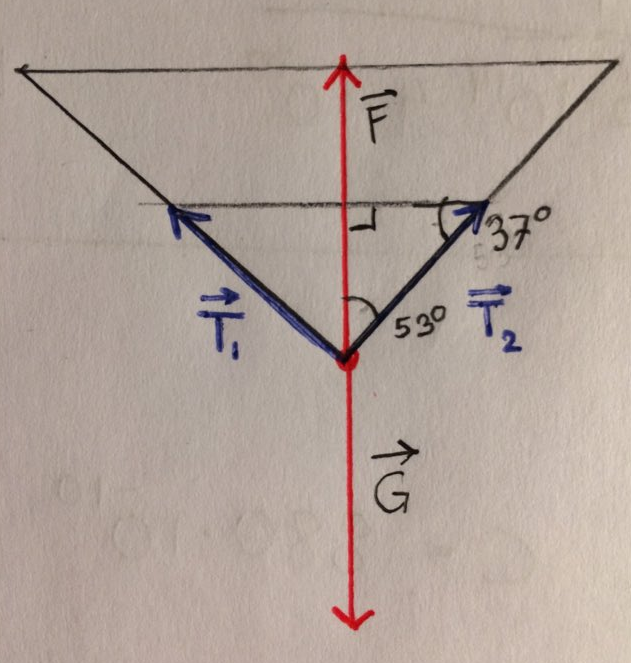
\includegraphics[width=50mm]{02_01}
    \end{center}
    \begin{equation}
      cos(\ang{53}) = \frac{mg/2}{T}
      \rightarrow T = \frac{mg}{2cos(\ang{53})}
    \end{equation}
    Snordraga $T = T_1 = T_2 = 181 N$

  \newpage

  \section*{Oppgåve 2}
    \subsection*{a)}
    Sidan kreftene $F_1$ og $F_2$ står horisontalt på systemet vil snordraget
    $T$ måtte stå for all krafta i y-retning.

    \begin{center}
      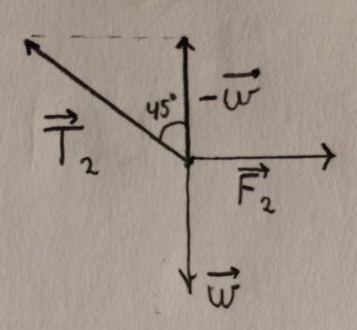
\includegraphics[width=55mm]{02_02a}
    \end{center}

    Dermed får vi ein likebeint trikant og kan bruke pythagoras
    \begin{equation}
      T = \sqrt{60,0^2 + 60,0^2} \rightarrow T = 84,9N
    \end{equation}

    \subsection*{b)}
    Vinkelen $\ang{45}$ sørger for at kreftene $w$ og $F_2$ er like store, 
    \begin{equation}
      |\vec{F_2}| = |\vec{w}| = 60,0N
    \end{equation}
    dersom kreftene $F_1$ og $F_2$ ikkje var like hadde ikkje 
    $\ang{90}$-forholdet vorte overholdt. Derfor er $F_1 = F_2 = 60,0N$

  \section*{Oppgåve 3}
    \subsection*{a)}

    \begin{center}
      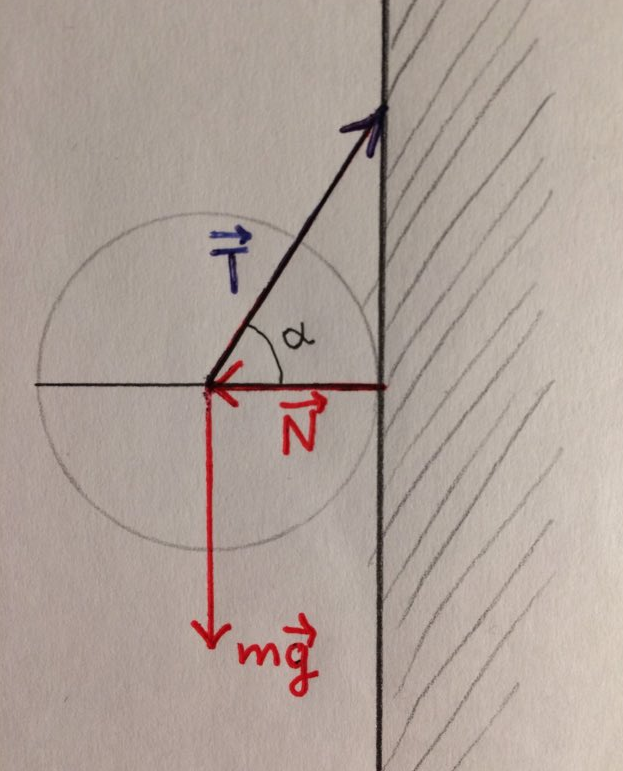
\includegraphics[width=50mm]{02_03a}
    \end{center}

    \subsection*{b)}
    Ballens tyngde er gitt ved
    \begin{equation}
      |m\vec{g}| = 45,0kg\cdot9,81m/s^2 = 441,5N
    \end{equation}
    vinkelen mellom snordraget $\vec{T}$ og normalkrafta frå veggen $\vec{N}$ er
    \begin{equation}
      cos \alpha = \frac{16,0}{30,0+16,0} \rightarrow \alpha = \ang{69,6}
    \end{equation}
    krafta til snordraget $\vec{T}$ er dermed gitt som
    \begin{equation}
      sin \alpha = \frac{|m\vec{g}|}{|\vec{T}|} \rightarrow
      T = \frac{441,5N}{sin(\ang{69,6})} = 471,0N
    \end{equation}

    \subsection*{c)}
    Vi kan finne normalkrafta frå veggen $N$
    \begin{equation}
      N^2 + G^2 = T^2 \rightarrow N = \sqrt{T^2 - G^2}
      \rightarrow |\vec{N}| = 164,1N
    \end{equation}
    sidan ballen står i ro i horisontal retning vil normalkrafta vere lik krafta
    frå ballen mot veggen.

  \section*{Oppgåve 4}
    Sidan vi antar at personen befinner seg i eit jamnt gravitasjonsfelt kan vi skrive
    tyngdekrafta på personen som $|m\vec{g}| = 70kg\cdot9,81m/s^2$. Summen av dei kjente 
    kreftene på heisen og personen er
    \begin{equation}
      \vec{N} - m\vec{g} = ma \rightarrow 72|\vec{g}| - 70|\vec{g}| = 70a
      \rightarrow a = \frac{72-70}{70}g = 0,28m/s^2
    \end{equation}
    heisen og personen er derfor i ein tilstand av positiv akselerasjon
    \begin{itemize}
      \item Dette utelukker \textbf{A} og \textbf{B}, som fordrer $a=0$.
      \item \textbf{D} er utelukka sidan det fordrer at $a<0$.
      \item \textbf{E} og \textbf{G} stemmer ikkje sidan $N>mg$
      \item Alternativer \textbf{C} og \textbf{F} kan stemme.
    \end{itemize}

  \section*{Oppgåve 5}
    Sidan klossen beveger seg med konstant fart er summen av kreftene
    langs skråplanet lik null
    \begin{center}
      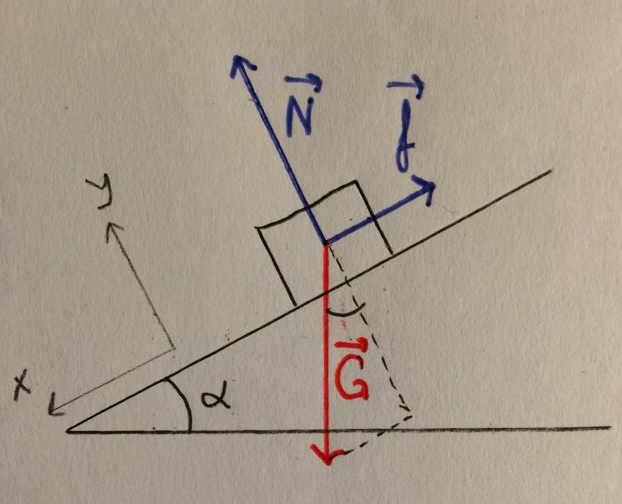
\includegraphics[width=73mm]{02_05}
    \end{center}
    \begin{equation}
      cos\alpha = \frac{N}{mg} \rightarrow N = mgcos\alpha
    \end{equation}
    \begin{equation}
      sin\alpha = \frac{f}{mg} \rightarrow f = mgsin\alpha
    \end{equation}
    \begin{equation}
      f = \mu N \rightarrow \mu = \frac{f}{N} = \frac{mgsin\alpha}{mgcos\alpha}
      \rightarrow \mu = \frac{sin\alpha}{cos\alpha} = tan\alpha
    \end{equation}
    Alternativ \textbf{G}

  \section*{Oppgåve 6}
    \begin{center}
      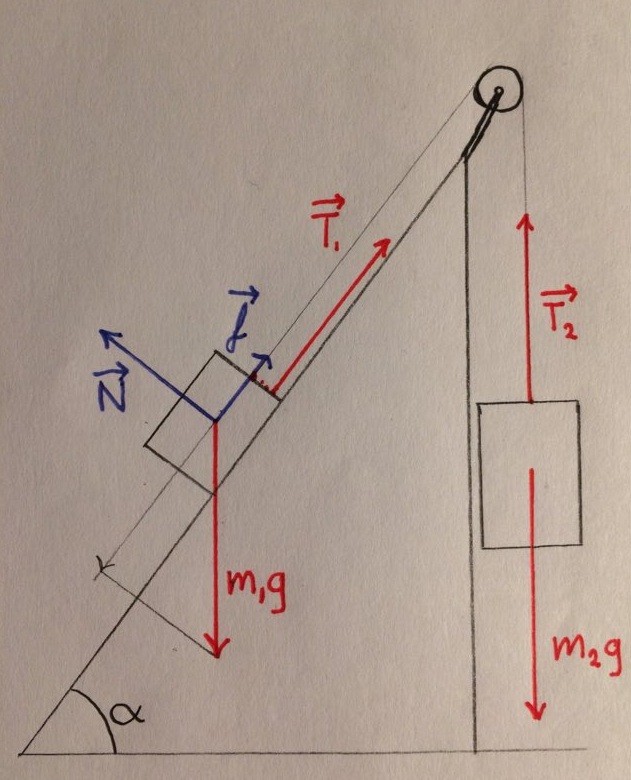
\includegraphics[width=63mm]{02_06}
    \end{center}
    \subsection*{a)}
    Eg byrjer med å dekomponere tyngdekrafta til $m_1$
    \begin{equation}
      sin\alpha = \frac{G_1}{m_1g} \rightarrow G_1 = m_1gsin\alpha
    \end{equation}
    normalkrafta tilsvarer y-komponenten til $m_1\vec{g}$
    \begin{equation}
      cos\alpha = \frac{N_1}{m_1g} \rightarrow N_1 = m_1gcos\alpha
    \end{equation}
    friksjonskrafta til $m_1$ er gitt ved
    \begin{equation}
      f = \mu N \rightarrow \mu m_1gcos\alpha
    \end{equation}
    summen av kreftene i systemet ved Newtons andre lov
    \begin{equation}
      \Sigma |\vec{F}| = G_2 - G_1 - f = ma \rightarrow
    \end{equation}
    \begin{equation}
      a = \frac{m_2g - m_1gsin\alpha - \mu m_1gcos\alpha}{m_2 + m_1} = 2,66m/s^2
    \end{equation}

    \subsection*{b)}
    Snordraga $T_1 = T_2$
    \begin{equation}
      T_1 = G_1 + f + m_1a = 257,4N
    \end{equation}

  \section*{Oppgåve 7}
    \subsection*{a)}
    \begin{center}
      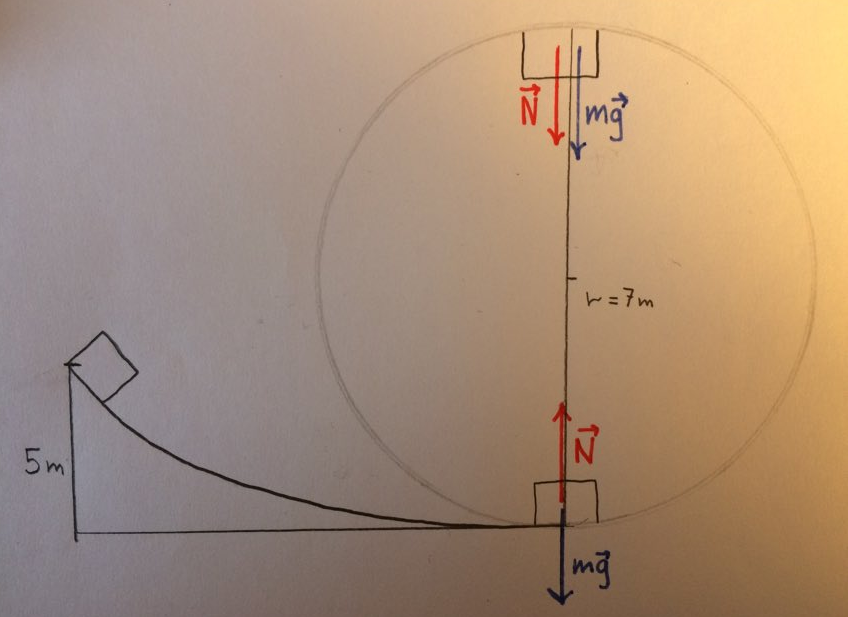
\includegraphics[width=73mm]{02_07}
    \end{center}
    Vi kjenner til at akselerasjonen i ein slik loop er gitt som
    \begin{equation}
      a = \frac{V^2}{R}
    \end{equation}

    \subsection*{b)}
    Når vogna er på botnpunktet i loopen er normalkrafta gitt ved
    \begin{equation}
      N = mg + m\frac{V^2}{R} = m \left( g + \frac{(70km/h)^2}{7m} \right)
      \rightarrow m \left( g + \frac{(19,4/h)^2}{7m} \right)
    \end{equation}
    \begin{equation}
      \rightarrow m(9,81N + 54,0N) = m\cdot 63,8
    \end{equation}
    som $G$ vert dette
    \begin{equation}
      63,8N/9,81N = 6,5G
    \end{equation}

    \subsection*{c)}
    For å finne $N$ må vi først finne farta på toppen, $V_2$. Vi kjenner til arbeid-
    /energiteoremet
    \begin{itemize}
      \item $W = K_2 - K_1$
      \item $K_1 = \frac{1}{2}mV_1^2$
      \item $K_2 = \frac{1}{2}mV_2^2$
    \end{itemize}
    setter inn for kjente størrelsar
    \begin{equation}
      -14mg = \frac{1}{2}mV_2^2 + \frac{1}{2}m19,4^2 \rightarrow
      V_2 = \sqrt{19,4^2 - 28g} = 10,1 m/s
    \end{equation}
    Når vogna er på toppunktet i loopen vil både normalkrafta og tyngdekrafta peke mot origo
    \begin{equation}
      N = m\frac{V^2}{R} - mg \rightarrow m \left( \frac{(10,1m/s)^2}{7m} - g \right)
      \rightarrow m(14,6N - 9,81N) = m4,76N
    \end{equation}
    som $G$ vert dette
    \begin{equation}
      4,76N/9,81N = 0,49G
    \end{equation}

    \subsection*{d)}
    Dersom normalkrafta $N=0$ vil vogna falle av banen.
    \begin{equation}
      \frac{V^2}{R} - g = 0 \rightarrow V = \sqrt{gR} = 8,3
    \end{equation}
    den minste farta vogna kan ha på toppunktet i loopen er derfor $8,3m/s$. Dermed må
    farta $v_0$ vere 
    \begin{equation}
      mg(5 - 14) = \frac{1}{2}m8,3^2 + \frac{1}{2}mv_0^2 \rightarrow
      v_0 = \sqrt{8,3^2 + 18g} = 15,7
    \end{equation}
    med farta $v_0 = 15,7 m/s$ skal vogna klare å komme seg igjennom loopen uten
    å falle ned frå banen.


  \section*{Oppgåve 8}
    Newtons tredje lov opprettholder at 
    \begin{equation}
      F_{a \rightarrow tau} = -F_{tau \rightarrow a}
    \end{equation}
    og at
    \begin{equation}
      F_{b \rightarrow tau} = -F_{tau \rightarrow b}
    \end{equation}
    men det trenger ikkje naudsynt vere tilfelle at
    \begin{equation}
      F_{b \rightarrow tau} = -F_{a \rightarrow tau}
    \end{equation}
    og denne skjevheten er opphavet til akselerasjonen.


\end{document}
